\section{Gerarchie di memoria}\label{capitolo6}
Per incrementare le performance di un computer bisogna considerare anche il suo sistema di memoria, bisogna infatti dare l'illusione di avere un sistema di memoria che sia simultaneamente ampio e veloce, inoltre bisogna fornire dati al processore ad alta frequenza.\\
Per fornire queste due caratteristiche dobbiamo sfruttare alcune caratteristiche, prima caratteristica da sfruttare è quella della \textbf{località}. La località è una caratteristica dei dati e può essere di due tipi:
\begin{description}
\item[Località temporale:] quando vi è un riferimento ad un elemento di memoria, la tendenza è quella di riferirsi allo stesso elemento nei momenti successivi (ad esempio in un loop).
\item[Località spaziale:] quando vi è un riferimento ad un elemento di memoria la tendenza è quella di accedere ai dati vicini nel tempo seguente, come nel caso di istruzioni sequenziali.
\end{description}
Un'altra soluzione è quella di sfruttare delle gerarchie di memoria come quelle mostrate in \figurename\,\ref{fig:gerarchia}, ogni livello di questa gerarchia ha dimensioni e velocità diverse implementate attraverso diverse tecnologie. Lo scopo è quello di fornire all'utente una grande quantità di memoria ad un costo contenuto ma fornendo comunque un tempo di accesso ridotto grazie alle tecnologie più veloci.
\begin{figure}[htb]
\centering
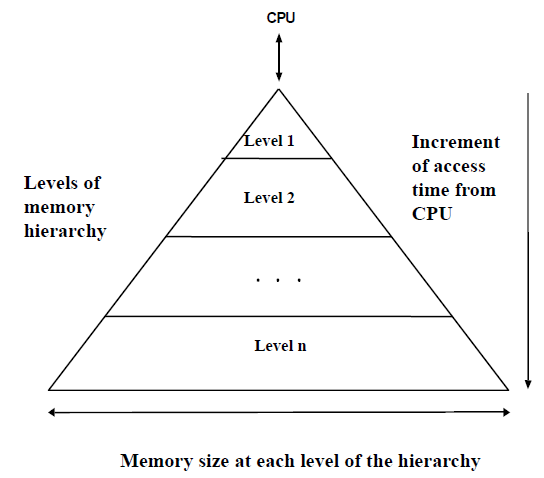
\includegraphics[scale=0.5]{img/gerarchia.png}
\caption{Esempio di gerarchia di memoria}\label{fig:gerarchia}
\end{figure}
\subsection{Caches}
La cache è un meccanismo che implementa i due obbiettivi prefissati, prima di tutto sfrutta entrambi i tipi di località, sfrutta la \emph{località temporale} mantenendo i dati acceduti più recentemente e sfrutta la \emph{località spaziale} prelevando dal livello superiore un blocco di dati nell'intorno del dato acceduto.
In \figurename\,\ref{fig:levelsmem} vediamo i livelli di caches e le gerarchie di memoria usati in due sistemi differenti, un sistema server ed un device mobile.
\begin{figure}[htb]
\centering
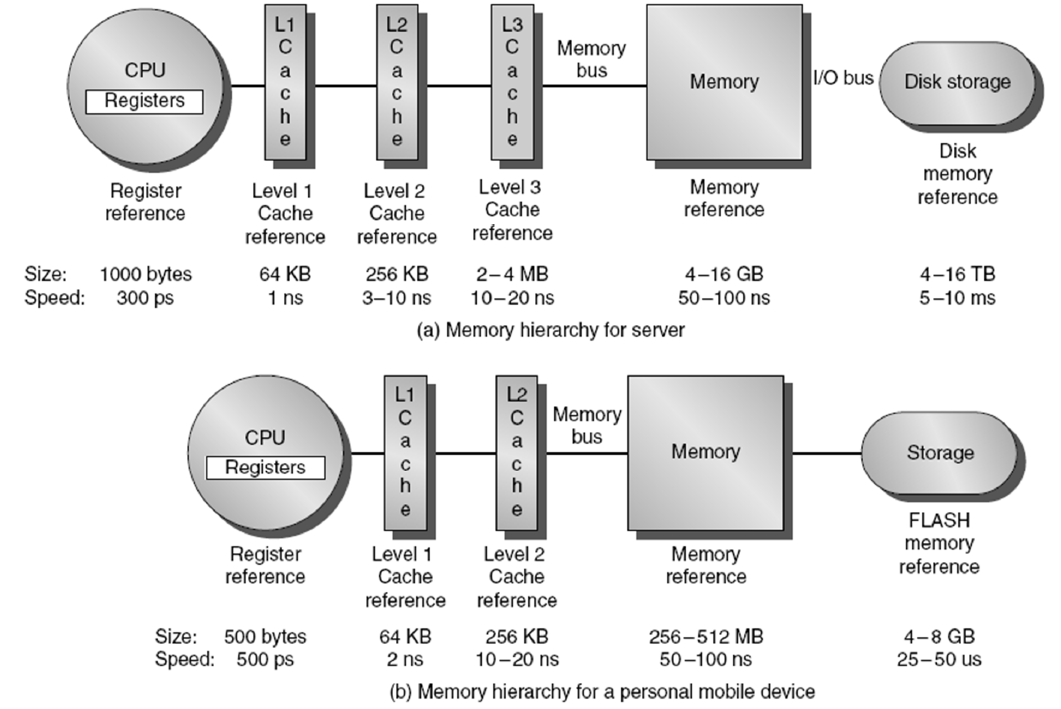
\includegraphics[scale=0.5]{img/levelsmem.png}
\caption{Sistema di memoria in un sistema server e in un device mobile.}\label{fig:levelsmem}
\end{figure}
Il design della gerarchia di memoria è diventato importante con i recenti processori multi-core, infatti la banda necessaria cresce con l'aumentare del numero di core, ad esempio un processore \emph{Core i7} alla frequenza di 3.2GHz genera due riferimenti a memoria per ogni core per clock che moltiplicati per i quattro core sono 25.6 miliardi di riferimenti a 64-bit al secondo più 12.8 miliardi di istruzioni a 128 bit per un totale di 409.6 GB/s. La banda di una memoria DRAM è di solo 25 GB/s ovvero il 6\% per implementare un sistema efficiente è perciò necessario avere una cache multiport, due livelli di cache per singolo core e un terzo livello di cache condiviso. Un esempio di tale sistema è mostrato in \figurename\,\ref{fig:i7cache}.
\begin{figure}[htb]
\centering
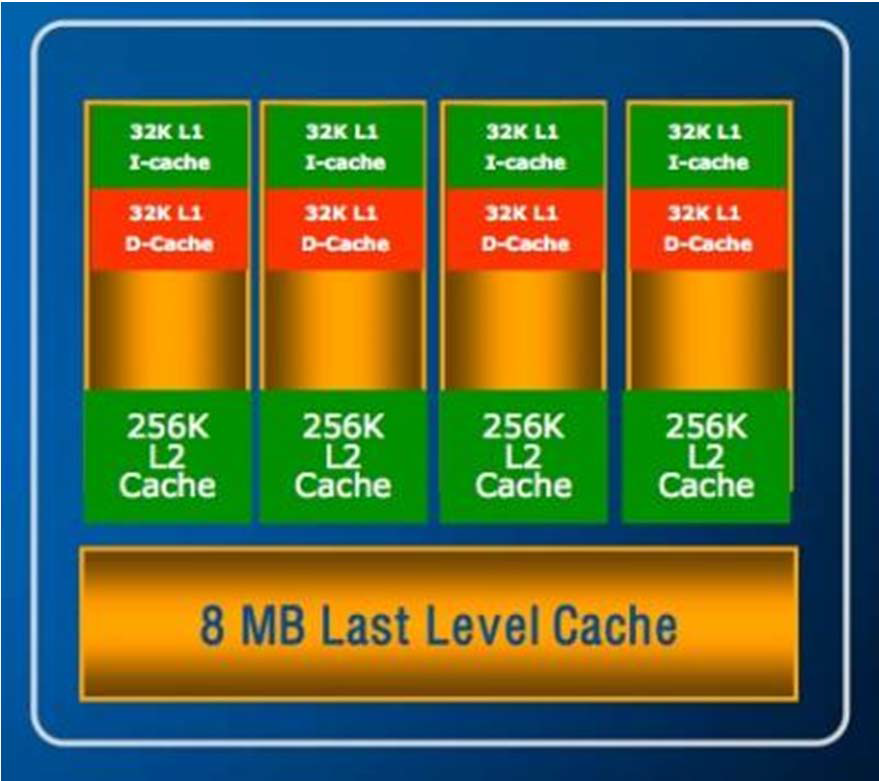
\includegraphics[scale=0.5]{img/i7cache.png}
\caption{Architettura cache di un processore Intel Core i7}\label{fig:i7cache}
\end{figure}
\subsubsection{Struttura e funzionamento di una cache}
Come abbiamo appena visto le gerarchie di memoria sono composte da diversi livelli i dati tuttavia sono copiati soltanto tra due livelli adiacenti. Per semplificare la nostra trattazione consideriamo soltanto due livelli, la cache e la memoria principale. La cache (livello \textbf{superiore}) è piccola e veloce ma molto costosa. La memoria centrale (livello \textbf{inferiore}) è di grandi dimensioni poco costosa e più lenta rispetto alla cache. La minima porzioni di dati che può essere copiata nella cache è chiamata \textbf{blocco} o \textbf{cache line}.
Per sfruttare la \emph{località spaziale} è necessario che la dimensione di un blocco sia un multiplo della dimensione di una parola. Per determinare il numero di blocchi che possono essere caricati in cache basta applicare la formula:
$$\# \ blocchi \ cache = cache \ size / block \ size$$
Di seguito alcune definizioni che ci aiuteranno nella nostra esposizione.
\paragraph{Cache Hit}
Si ha un \emph{cache hit} se ad una richiesta di dati si trova il dato già presente in cache.
\paragraph{Cache Miss}
Quando si richiede un dato ma tale dato non è presente in nessun blocco di cache allora si ha un \emph{cache miss}. Per trovare tale blocco è necessario accedere al livello che sta più in basso nella gerarchia di memoria. In caso di miss è necessario bloccare la CPU e richiedere il blocco alla memoria centrale, copiare il blocco in cache e poi ripetere l'accesso alla cache per effettuare uno \emph{hit.}
\paragraph{Hit Rate}
L'\emph{hit rate} è il numero di accessi in memoria che trovano il dato in cache rispetto al numero di accessi totali.
$$Hit \ Rate = \frac{ \# Hit}{\# \ Memory \ Accesses}$$
\paragraph{Hit Time}
L'\emph{hit time} è il tempo necessario per per accedere al dato quando esso è presente nel livello più alto della cache, questo tempo include il tempo per decidere se il dato è presente.
\paragraph{Miss Rate}
Il \emph{miss rate} è il numero di accessi a memoria che non trovano il dato nel livello più alto e che quindi necessitano di un accesso ad un livello più basso di memoria rispetto al numero di accesso totali. Data questa definizione abbiamo che:
$$Miss \ Rate + Hit \ Rate = 1$$
\paragraph{Miss Penality}
Il \emph{miss penality} è il tempo necessario per accedere al livello inferiore della memoria e rimpiazzare il blocco contenente il dato al livello superiore.
\paragraph{Miss Time}
Tempo totale per accedere ad un dato che non si trova nel livello più alto della cache è dato da:
$$Miss \ Time = Hit \ Time + Miss \ Penality$$
\paragraph{Tempo medio di accesso}
Il \emph{tempo medio di accesso} alla memoria (AMAT) è dato dalla percentuale di hit per il tempo di accesso più la percentuale di miss per il relativo tempo di accesso. 
$$AMAT = Hit \ Rate * Hit \ Time + Miss \ Rate * Miss \ Time$$
Dato che
$$Miss \ Time = Hit \ Time + Miss \ Penality$$
e
$$Miss \ Rate + Hit \ Rate = 1$$
allora possiamo scrivere il tempo medio di accesso come:
$$AMAT = Hit \ Time + Miss \ Rate * Miss \ Penality$$
Analizziamo ora come sono strutturate le cache e le loro tecnologie di implementazione.
Innanzitutto ogni record di una cache contiene:
\begin{description}
\item[Bit di validità:] per indicare se la posizione corrente contiene dei dati validi oppure no, durante il \emph{bootstrap} del sistema tutti i record vengono marchiati come \emph{invalidi.}
\item[Tag:] Questo campo contiene un valore che identifica inequivocabilmente l'indirizzo di memoria corrispondente ai dati immagazzinati.
\item[Data:] Contiene una copia dei dati della memoria.
\end{description}
Tale struttura è rappresentata in \figurename\,\ref{fig:cachestruct}.
\begin{figure}
\centering
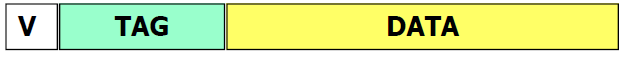
\includegraphics[scale=0.4]{img/cachestruct.png}
\caption{Struttura di un record di cache}\label{fig:cachestruct}
\end{figure}
Esistono tre metodi per implementare un sistema di cache, essi sono rispettivamente la cache \emph{direct map}, la cache \emph{fully associative} e la cache \emph{associativa a n vie}. Questa distinzione di tipologie è dovuta al problema del \textbf{piazzamento dei blocchi} ovvero come assegnare la posizione in memoria cache ad un blocco che viene caricato in memoria centrale.
\paragraph{Cache direct map}
Nelle cache di tipo \emph{direct map} ogni indirizzo di memoria corrisponde ad uno ed un solo blocco in cache tale blocco di cache è determinato da:
$$(Block \ Address)_{cache} = (Block \ Address)_{mem} \ mod \ (\# \ cache \ blocks)$$
Un esempio di tale meccanismo è mostrato in \figurename\,\ref{fig:directmapexe}
\begin{figure}
\centering
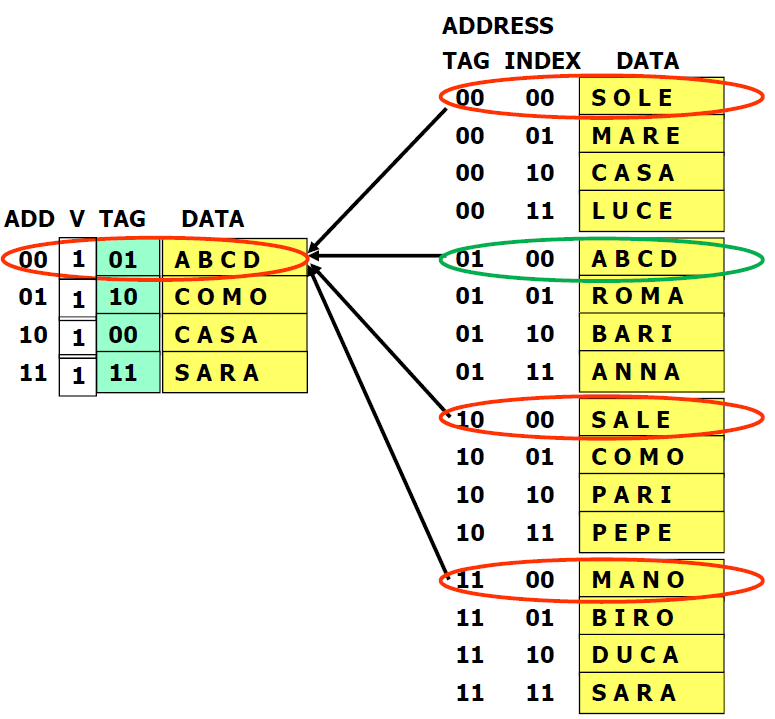
\includegraphics[scale=0.5]{img/directmapexe.png}
\caption{Esempio di piazzamento di blocchi nel caso di cache di tipo direct map}\label{fig:directmapexe}
\end{figure}
L'indirizzamento avviene nel modo descritto dalla \figurename\,\ref{fig:directaddressing} dove dato un indirizzo di \emph{N bit} viene suddiviso in 4 campi:
\begin{description}
\item[Byte offset:] che serve ad identificare il byte dato all'interno della parola, nel caso in cui la memoria non sia indirizzabile al byte allora $B = 0$
\item[Byte offset:] che serve ad identificare la parola all'interno del blocco , nel caso in cui il blocco abbia dimensione di una parola allora $K = 0$
\item[Index:] identifica il blocco tramite \textbf{M} bit, dove 
$$M = \log_2 \# \ Block$$
\item[Tag:] necessario per comparare il blocco selezionato tramite l'index, la dimensione del tag è data da:
$$N - (M + K + B)$$
\end{description}
\begin{figure}
\centering 
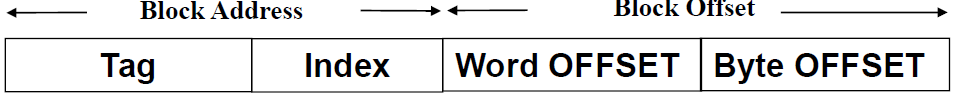
\includegraphics[scale=0.5]{img/directaddressing.png}
\caption{Indirizzamento in un sistema di cache direct map}\label{fig:directaddressing}
\end{figure}
\paragraph{Cache completamente associativa}
In una cache di tipo \emph{fully associative} un blocco di memoria può essere posizionato in un qualsiasi blocco cache, durante la ricerca di un blocco tutti i blocchi cache vengono controllati e il loro campo \emph{tag} viene comparato con quello del blocco da cercare. Il campo index non esiste nella cache completamente associativa.
I campi che compongono un record in una cache completamente associativa sono mostrati in \figurename\,\ref{fig:fullyaddressing} e sono rispettivamente:
\begin{description}
\item[Byte offset:] che serve ad identificare il byte dato all'interno della parola, nel caso in cui la memoria non sia indirizzabile al byte allora $B = 0$
\item[Byte offset:] che serve ad identificare la parola all'interno del blocco , nel caso in cui il blocco abbia dimensione di una parola allora $K = 0$
\item[Tag:] Serve ad identificare il blocco in cache ed è uguale a 
$$N - (B + K)$$
\end{description}
\begin{figure}[htb]
\centering
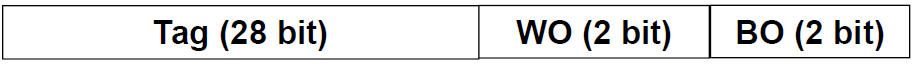
\includegraphics[scale=0.5]{img/fullyaddressing.png}
\caption{Campi di una cache completamente associativa}\label{fig:fullyaddressing}
\end{figure}
Un esempio di cache completamente associativa è mostrato in \figurename\,\ref{fig:fullyexemp}
\begin{figure}[htb]
\centering
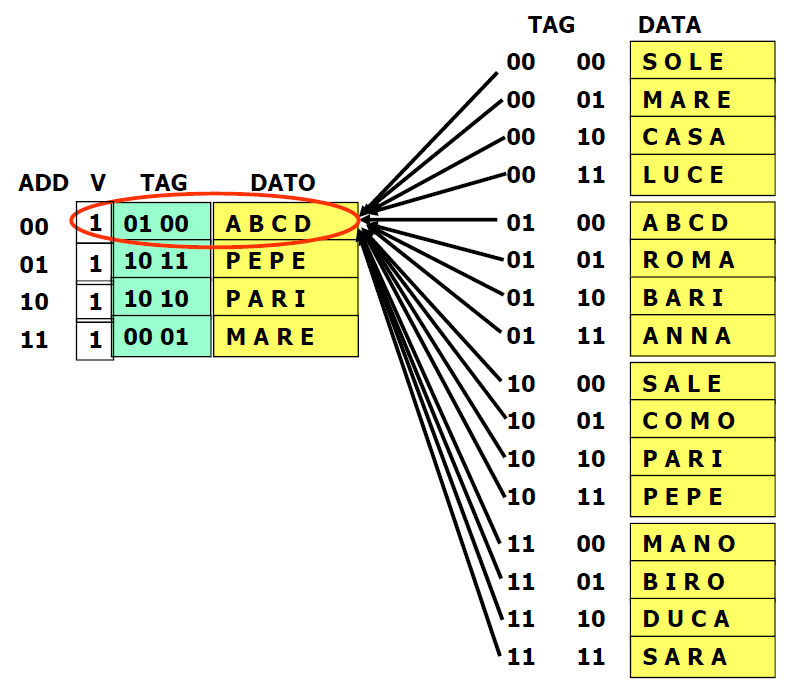
\includegraphics[scale=0.5]{img/fullyexemp.png}
\caption{Esempio di una cache completamente associativa}\label{fig:fullyexemp}
\end{figure}
\paragraph{Cache associativa ad \emph{n} vie}
In questo caso la cache è composta da dei \emph{set} ed ogni set è composto da un determinato numero di blocchi.
$$\# \ Blocchi = Cache \ size / Block \ size$$
$$\# \ Sets = Cache \ size / (Block \ size * n)$$
Un blocco di memoria può essere posto in uno qualsiasi dei blocchi di un set e la ricerca deve avvenire in tutti i blocchi di quel set. Per calcolare in quale set un blocco dovrà essere posizionato bisogna utilizzare la formula:
$$(Set)_{cache} = (Block \ address)_{mem} \ mod \ (Num \ sets \ in \ cache)$$
Un esempio di utilizzo di una cache set associativa è mostrato in \figurename\,\ref{fig:setexemp}
\begin{figure}[htb]
\centering
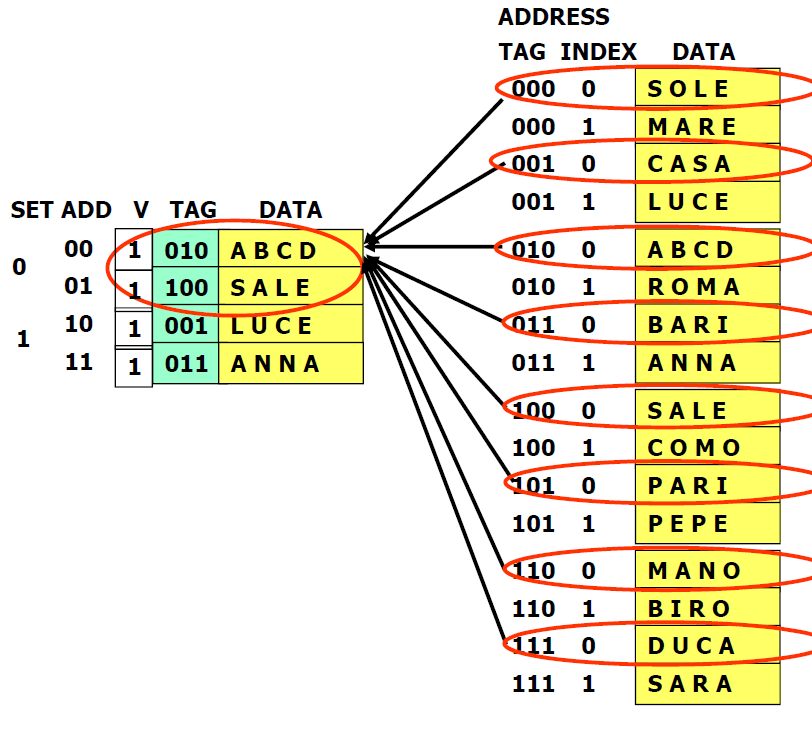
\includegraphics[scale=0.5]{img/setexemp.png}
\caption{Esempio di una cache associativa a due vie}\label{fig:setexemp}
\end{figure}
L'indirizzamento in una cache associativa ad n vie avviene come nel caso di cache di tipo direct map ma questa volta il campo index serve ad identificare il set nel quale effettuare la ricerca del blocco come mostrato in \figurename\,\ref{fig:setaddressing}
\begin{figure}[htb]
\centering
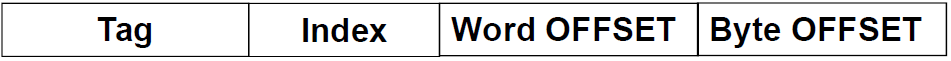
\includegraphics[scale=0.5]{img/setaddressing.png}
\caption{Indirizzamento in una cache associativa a due vie}\label{fig:setaddressing}
\end{figure}
Il problema principale che si ha quando si utilizza un meccanismo di cache è quello di decidere dove posizionare i blocchi di memoria quando questi sono copiati in cache in quanto la memoria è molto più grande di quella cache. I tre meccanismi di cache che abbiamo appena visto risolvono questo problema in modi diversi come possiamo vedere dalla 	\figurename\,\ref{fig:tipicache}. Come vediamo nel caso di completamente associativa il blocco può essere posizionato in qualsiasi blocco cache, questo significa che per verificare che un blocco sia già presente in cache bisogna controllare tutti i blocchi della cache aumentando così il tempo di servizio. Nel caso di cache \emph{direct map} il blocco può essere posizionato in un solo blocco di cache questo fa si che la ricerca sia molto veloce ma può portare ad altri problemi (cosa succede se il blocco 4 contiene delle istruzioni che sono contenute nel blocco 12?). Nel caso di cache associativa a $n$ vie abbiamo una via di mezzo tra le precedenti infatti il blocco può essere posizionato in qualsiasi blocco all'interno del set ma la ricerca avviene soltanto all'interno del set e non su tutta la cache.
\begin{figure}[htb]
\centering
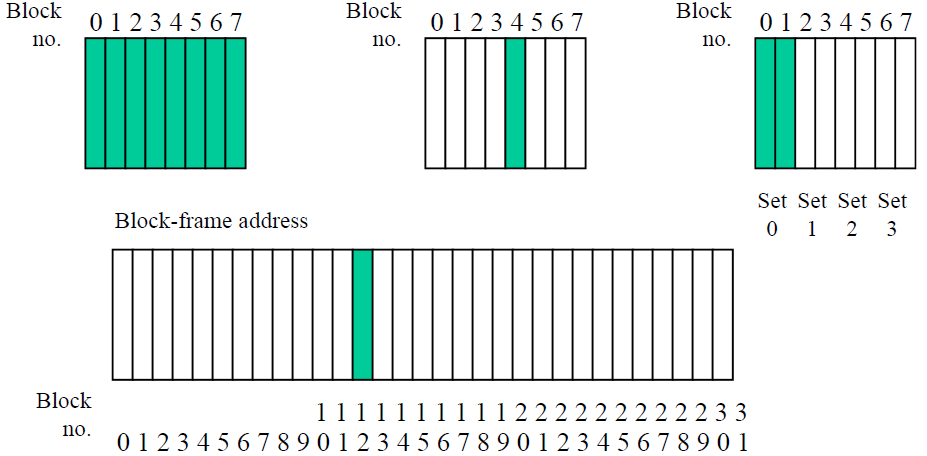
\includegraphics[scale=0.5]{img/tipicache.png}
\caption{Problema del \emph{block placement} nei tre meccanismi di cache}\label{fig:tipicache}
\end{figure}
La soluzione al problema del piazzamento dei blocchi sembrerebbe allora quello dell'incremento del livello di associatività. Tuttavia pur riducendo il \emph{miss rate} aumentano in modo esponenziale i costi di implementazione ed inoltre incrementa anche il tempo di \emph{hit}. La decisione di quale tecnologia utilizzare dipende dal tradeoff di costi e riduzione di \emph{miss rate.}\\
In caso di miss dobbiamo decidere quale blocco sostituire, in caso di completamente associativa i blocchi candidati sono tutti mentre nel caso di set associativa i blocchi candidati sono soltanto quelli del set corrispondente al blocco da inserire. Esistono diverse strategie per effettuare la selezione e sono:
\begin{itemize}
\item Random o pseudo random
\item LRU (Least Recently Used)
\item FIFO (First In First Out)
\end{itemize}
Un altro problema che si viene a creare quando dobbiamo sostituire un blocco è quello della \emph{write policy} ovvero come ci dobbiamo comportare se il blocco che stiamo sostituendo è stato modificato. Esistono due tecniche principali:
\begin{description}
\item[Write-through:] in questo caso ad ogni scrittura vengono aggiornati sia il blocco in cache che il blocco in memoria, questo meccanismo ci permette di non preoccuparci della sostituzione ed è di facile implementazione, tuttavia richiede la presenza di un \emph{write buffer} come quello in \figurename\,\ref{fig:writebuffer}. 
\item[Write-back:] questo meccanismo prevede che le modifiche ad un blocco siano scritte solamente in cache e tali modifiche siano scritte in memoria centrale solo quando il blocco in cache viene sostituito, per implementare questo meccanismo è necessario aggiungere ai campi della cache un \emph{dirty bit} che indica se il blocco è stato modificato durante la sua permanenza in cache.
Questo meccanismo permette scritture più veloci e anche scritture multiple su uno stesso blocco richiedono un unica scrittura in memoria centrale.
\end{description}
\begin{figure}[htb]
\centering
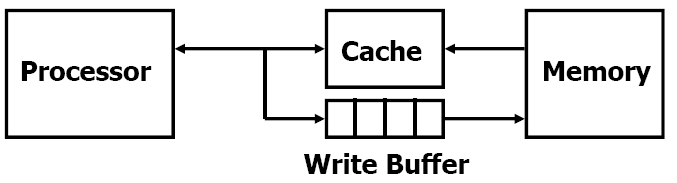
\includegraphics[scale=0.5]{img/writebuffer.png}
\caption{Utilizzo del write buffer}\label{fig:writebuffer}
\end{figure}
Per implementare un meccanismo di \emph{write-through} efficace abbiamo visto come sia necessario un \emph{write buffer}, ovvero un buffer di tipo FIFO che permette al processore di non attendere i tempi di scrittura della memoria. Il processore scrive i dati in cache e nel write buffer, un controllore scrive i dati del buffer nella memoria più bassa. Il problema della scrittura tuttavia non è ancora risolto in quanto il buffer si può saturare e a quel punto è necessario bloccare il processore in attesa della scrittura.\\
La scrittura di dati in memoria presenta un ulteriore problema, infatti può capitare che sia necessario scrivere su di un blocco che non è presente in cache, anche per questo caso esistono due soluzioni distinte:
\begin{description}
\item[Write allocate:] in questo caso prima di scrivere il dato viene allocato in cache il blocco corrispondente allo spazio di memoria che dovrebbe essere scritto e la scrittura avviene sul blocco appena allocato.
\item[No write allocate:] in questo caso il dato da scrivere viene semplicemente inviato alla memoria di più basso livello senza allocare nuovi dati in cache.
\end{description}
Le tecniche di \emph{write-back} o \emph{write-through} e quelle di \emph{write allocate} e di \emph{no write allocate} possono teoricamente essere combinate in qualsiasi modo, ma in pratica si utilizzano solo le combinazioni \emph{write-back} e \emph{write allocate} e \emph{write-through} con \emph{no write allocate}.
\subsubsection{Analisi delle performance}\label{cachel2}
Come abbiamo visto nei capitoli precedenti abbiamo che 
$$CPU_{time} = (CPU_{exec-cycles} + Memory \ stall \ cycle) \times T_{CLK}$$
dove:
\begin{description}
\item[$T_{CLK}$:] periodo di tempo del clock
\item[$CPU_{exec-cycles}$:] $IC \times CPI_{exec}$
\item[$IC$:] Instruction count
\item[$Memory \ stall \ cycle$:] $IC \times Miss \ per \ instr \times Miss \ penality$
\end{description}
A questo punto possiamo riscrivere la precedente equazione come:
$$IC \times (CPI_{exec} + Miss \ per \ instr \times Miss \ penality) \times T_{CLK}$$
dove 
$$Miss \ per \ instr = Memory Access Per Instrunction \times Miss \ Rate$$
$$IC \times (CPI_{exec} + MAPI \times Miss \ Rate \times Miss \ penality) \times T_{CLK}$$
Questa formula non tiene conto degli stalli dovuti ai conflitti della pipeline ma solo di quelli dovuti all'accesso in memoria ma sono questi quelli importanti per la nostra trattazione.\\
A questo punto vogliamo ridurre il tempo di accesso ai dati ovvero ridurre \emph{AMAT}
$$AMAT = Hit \ Time + Miss \ Rate * Miss \ Penality$$
questo significa ridurre uno dei tre componenti della formula, lo \emph{hit time}, il \emph{miss rate} o il \emph{miss penality}. Per fare ciò introduciamo un secondo livello di cache, il primo livello (L1) abbastanza veloce da soddisfare il più veloce ciclo di clock, il secondo livello (L2) grande abbastanza da catturare la maggior parte degli accessi destinati alla memoria in modo da ridurre gli effetti del miss penality. Il tempo medio di accesso per quanto riguarda il primo livello di cache è dato da:
$$AMAT = Hit \ Time_{L1} + Miss \ Rate_{L1} \times Miss \ Penality_{L1}$$
dove il \emph{miss penality} è dato da:
$$Miss \ Penality_{L1} = Hit \ Time_{L2} + Miss \ Rate_{L2} \times Miss \ Penality_{L2}$$
Otteniamo così che il tempo medio di accesso con due livelli di cache è dato da 
$$AMAT = Hit \ Time_{L1} + Miss \ Rate_{L1} \times (Hit \ Time_{L2} + Miss \ Rate_{L2} \times Miss \ Penality_{L2})$$
Possiamo però fare una distinzione tra i miss rate possiamo definire un \textbf{local miss rate} ed un \emph{global miss rate}.
Per calcolare un \emph{local miss rate} si calcolano il numero di miss nel livello di cache in esame diviso il numero di accessi in quel livello di cache otteniamo così un \emph{miss rate} per L1 e un \emph{miss rate} per L2. Nel caso di \emph{global miss rate} invece si calcolano il numero di miss in quel livello di cache diviso il numero totale di accessi a memoria generati dalla CPU. Per il livello L1 il \emph{miss rate} coincide con quello locale mentre per il livello L2 abbiamo che $Miss \ Rate_{L1L2} = Miss \ Rate_{L1} \times Miss \ Rate_{L2}$. Il miss rate di tipo globale è una misura più veritiera di quanti accessi a memoria effettuati dalla CPU arrivano realmente alla memoria centrale. Possiamo così riscrivere il tempo medio di accesso come:
$$AMAT = Hit \ Time_{L1} + Miss \ Rate_{L1} \times Hit \ Time_{L2} + Miss \ Rate_{L1L2} \times Miss \ Penality_{L2}$$
A questo punto possiamo analizzare l'impatto dei memory miss sul tempo di esecuzione, questo impatto è dato da 
$$CPU_{time} = IC \times (CPI_{exec} + MAPI \times MR_{L1} \times HT_{L2}+ MAPI \times MR_{L1L2} \times MP_{L2}) \times T_{CLK}$$
\subsection{Incremento delle performance}
Fino ad ora abbiamo visto come sono costruite e come funzionano le diverse tipologie di cache, ora ci chiediamo come incrementarne le performance. Partendo dal tempo medio di accesso a memoria:
$$AMAT = HT + MR * MP$$
Da questa formula vediamo che per ridurre il tempo di accesso a memoria possiamo ottimizzare uno dei tre fattori ovvero:
\begin{itemize}
\item Ridurre il \emph{miss rate}
\item Ridurre il \emph{miss penality}
\item Ridurre lo \emph{hit time}
\end{itemize}
\paragraph{Cache miss}
Prima di iniziare la nostra trattazione vediamo quali tipi di cache miss possiamo incontrare, possiamo distinguerne quattro tipologie:
\begin{itemize}
\item Compulsory Misses
\item Capacity Misses
\item Conflict Misses
\item Coherence Misses
\end{itemize}
La \emph{compulsory misses} si ha all'avvio di un programma o del calcolatore quando tutti i blocchi di cache sono segnati come invalidi e per questo ogni nuovo caricamento di un blocco porta ad un miss.
La \emph{capacity misses} si ha quando la cache non è in grado di contenere tutti i blocchi necessari all'esecuzione tale tipo di miss decresce con l'aumentare della capacità della cache.
La \emph{conflic misses} avviene solo nel caso in cui la cache sia di tipo direct map o set associative ed avviene perché un blocco appena eliminato per far spazio ad un altro blocco sarà necessario nel breve periodo; tale miss è anche chiamata \emph{collision misses}.
L'ultima tipologia di miss è relativamente nuova ed è causata da problemi di coerenza tra cache in un ambiente multiprocessore.
\subsubsection{Ridurre il miss rate}
Per ridurre il miss rate in molti casi basta ridurre le capacity miss, il modo più semplice per farlo è aumentare la dimensione della cache, tuttavia questo incrementa il tempo di hit nonché l'area e il consumo di energia.\\
Un altro metodo è quello di incrementare la dimensione dei blocchi di cache, così facendo si sfrutta maggiormente la località spaziale, tuttavia aumentando troppo la dimensione del blocco si ottiene l'effetto opposto aumentando il miss rate inoltre l'aumento della dimensione del blocco di cache aumenta il miss penality e riduce il numero di blocchi disponibili aumentando la possibilità di \emph{conflict misses}.\\
Per ridurre la possibilità di \emph{conflict misses} si può aumentare l'associatività della cache tuttavia questo comporta un aumento di logica con conseguente aumento dell'area di silicio e del consumo di energia, inoltre si ha anche un aumento del tempo di \emph{hit}.\\
Un problema di difficile risoluzione è quello di ridurre i \emph{conflict miss} mantenendo ridotti i tempi di hit come nel caso di cache \emph{direct map}. Una soluzione è quella di introdurre un buffer nel quale immagazzinare i blocchi scartati dalla cache in modo da migliorare l'utilizzo della località temporale. Tale buffer viene chiamato victim cache ed è una cache di tipo completamente associativo di piccole dimensioni, infatti una victim cache di soli 4 registri associata ad una cache direct map di 4KB riduce fino al 95\% dei conflitti. Il funzionamento della \emph{victim cache} è molto semplice essa è situata tra la cache e il suo percorso di caricamento, ogni volta che avviene un miss si controlla se nella victim cache è presente il blocco mancante prima di inoltrare la richiesta al livello più basso. Nel caso in cui il blocco sia presente nella victim cache avviene una sostituzione tra un blocco in cache e il blocco necessario nella victim cache.\\
Analizziamo ora due metodi che ci permettono di ottenere un breve tempo di hit mantenendo comunque un livello di miss da conflitto dell'ordine di una cache a due vie, il primo meccanismo si applica alle cache di tipo \emph{direct map} e viene denominato \emph{divide cache}, quando avviene un miss si controlla l'altra metà della cache. Il secondo metodo denominato \emph{way prediction} si applica alle cache di tipo associativo a due vie e consiste nell'utilizzare un bit extra per predire quale via sarà intrapresa durante il prossimo accesso in cache in modo da pre settare il multiplexer e ridurre i tempi di accesso, in caso la predizione sia corretta si ottiene un tempo di accesso pari allo \emph{hit time} in caso di predizione sbagliata abbiamo un tempo di accesso più lento. Questa tecnica oltre a ridurre il tempo di accesso riduce anche il consumo di energia. Tuttavia questo meccanismo è efficace per le cache che non sono a diretto contatto con il processore in quanto uno \emph{slow hit} degrada notevolmente le performance, inoltre tale tecnica è efficace se si ha un buon predittore e quindi il numero di predizioni corrette è maggiore di quelle sbagliate altrimenti le performance degradano sensibilmente.\\
Un altro modo per ridurre il tempo di hit e il miss rate è quello di utilizzare delle tecniche hardware di \emph{pre-fetching} ovvero la possibilità di prelevare più di un blocco nell'istante di prelevamento , questo meccanismo aumenta virtualmente la banda disponibile tuttavia nel caso vi sia un interferenza tra \emph{pre-fetching} e misses si ha un degrado delle performance. Un esempio dei vantaggi di questa tecnica è mostrato in \figurename\,\ref{fig:prefetchingcache} nella quale si mostra l'incremento di performance grazie al prelevamento di due blocchi quando avviene un miss (includendo il blocco sequenzialmente successivo).
\begin{figure}
\centering
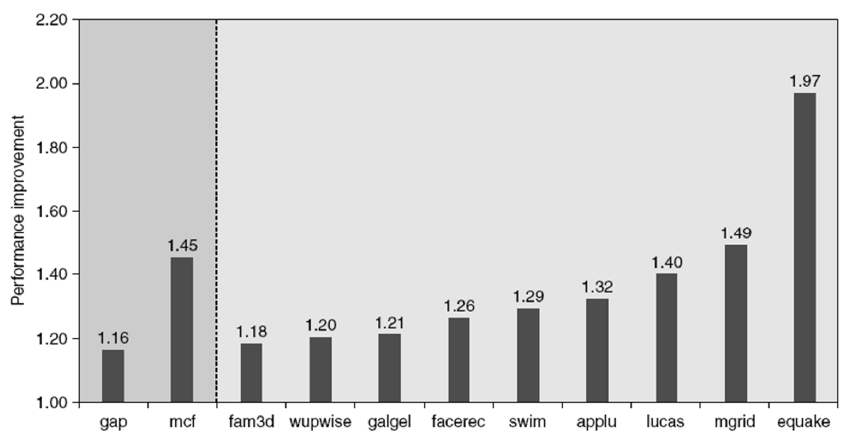
\includegraphics[scale=0.5]{img/prefetchingcache.png}
\caption{Incremento di performance dovuto al pre-fetching di due blocchi quando avviene un miss}\label{fig:prefetchingcache}
\end{figure}
Una tecnica simile è quella del \emph{software pre-fetching} ovvero il compilatore inserisce delle istruzioni dette di pre-fetching per richiedere dei dati prima che essi siano necessari. Questo meccanismo può essere di due tipi:
\begin{description}
\item[Register prefetch:] i dati vengono caricati nei registri
\item[Cache prefetch:] i dati vengono caricati in cache
\end{description}
Tuttavia questa tecnica è efficace solo se il costo in termini di tempo di esecuzione e aumento della complessità del codice è minore del vantaggio che si ha in termini di riduzioni di misses.\\
Esiste, infine un ramo di ottimizzazioni che riguardano la riduzione dei misses tramite l'utilizzo di tecniche di ottimizzazione effettuate dal compilatore.
Tali tecniche sono:
\begin{description}
\item[Mearging arrays:] che permette di incrementare la località spaziale di una struttura di elementi rispetto a due array.
\item[Loop Interchange:] incrementa la località spaziale scambiando l'innestamento dei loop per permettere un accesso ai dati in modo più continuo.
\item[Loop Fusion:] incrementa la località spaziale combinando due cicli indipendenti che eseguono lo stesso loop su alcune variabili sovrapposte.
\item[Bloccking:] incrementa la località temporale tramite l'accesso a blocchi di dati ripetutamente al posto di accedere per righe o per colonne.
\end{description}
Un esempio di \emph{mearging array} è mostrato in \figurename\,\ref{fig:meargingarray} nel quale si riducono i conflitti tra le variabili \texttt{val} e \texttt{key} incrementando la località spaziale
\begin{figure}[htb]
\centering
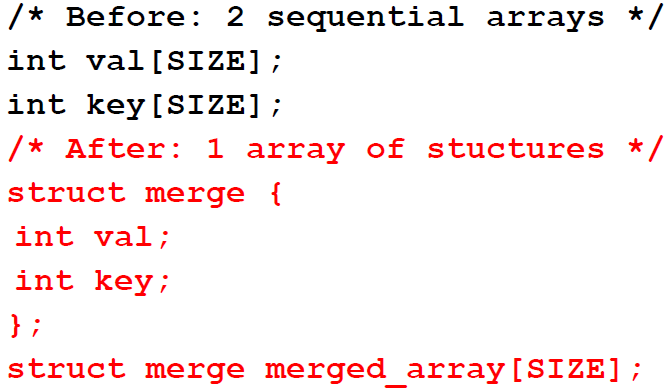
\includegraphics[scale=0.5]{img/meargingarray.png}
\caption{Esempio di mearging array}\label{fig:meargingarray}
\end{figure}
Un esempio di \emph{loop interchange} è mostrato in \figurename\,\ref{fig:loopinterchange} nel quale si ha un accesso a memoria con un avanzamento di 100 parole anziché 5000 aumentando così la località spaziale.
\begin{figure}[htb]
\centering
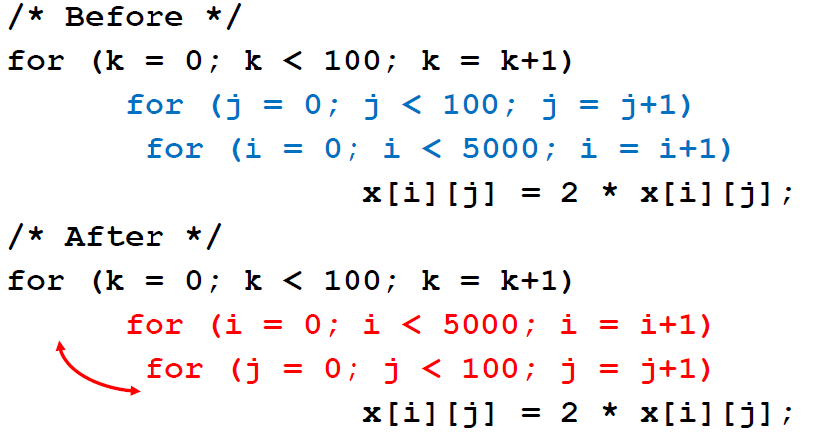
\includegraphics[scale=0.5]{img/loopinterchange.png}
\caption{Esempio di loop interchange}\label{fig:loopinterchange}
\end{figure}
Nell'esempio di \figurename\,\ref{fig:loopfusion} viene mostrato come incrementare la località spaziale tra due cicli che lavorano su alcune variabili comuni.
\begin{figure}[htb]
\centering
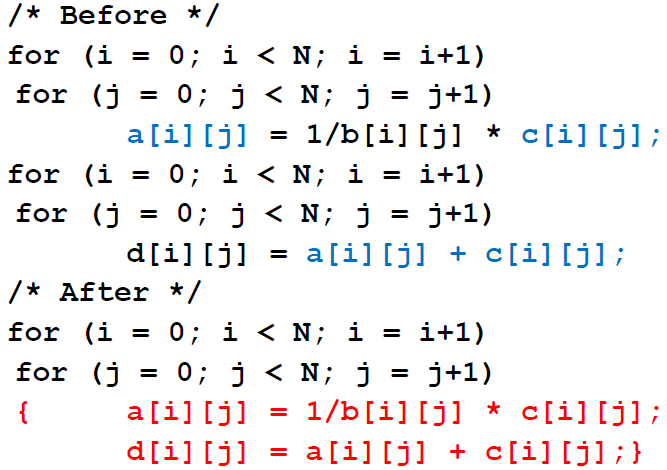
\includegraphics[scale=0.5]{img/loopfusion.png}
\caption{Esempio di loop fusion}\label{fig:loopfusion}
\end{figure}
Per quanto riguarda il \emph{blocking} la \figurename\,\ref{fig:blockingb} e \ref{fig:blockinga} mostrano come si effettua un blocking ovvero si modifica l'accesso ad una matrice non più per righe o colonne ma tramite dei blocchi, tale meccanismo richiede più memoria ma migliora la località spaziale, nell'esempio il fattore \emph{B} è chiamato \emph{fattore di blocco}.
\begin{figure}[htb]
\subfigure[blocking before]{
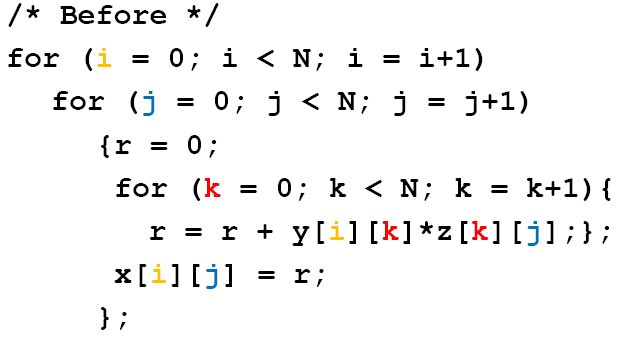
\includegraphics[scale=0.45]{img/blockingb.png}
\label{fig:blockingb}
}
\subfigure[blocking after]{
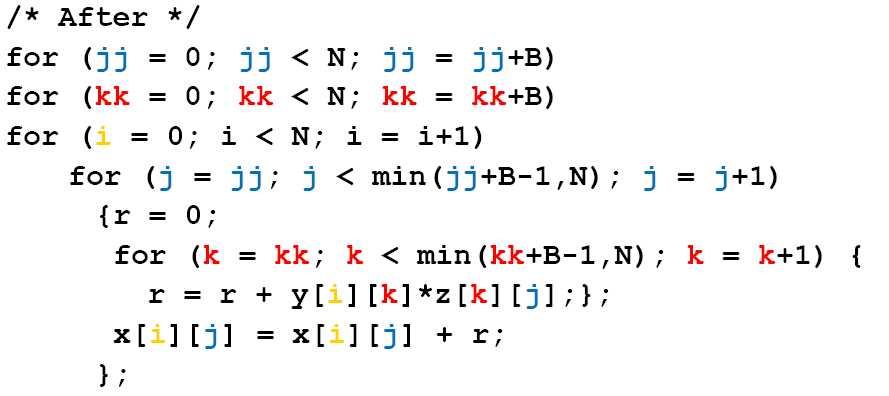
\includegraphics[scale=0.45]{img/blockinga.png}
\label{fig:blockinga}
}
\caption{Esempio di utilizzo del blocking}
\end{figure}
\subsubsection{Ridurre il miss penality}
Come per il \emph{miss rate} anche per il \emph{miss penality} esistono diverse tecniche per la riduzione di questo fattore.  La prima tecnica che analizziamo è denominata \emph{read priority} e si basa sull'idea di dare una maggiore priorità ai miss che riguardano un dato in lettura rispetto a dei miss che riguardano una scrittura, per implementare questa tecnica è necessario dimensionare adeguatamente il \emph{write buffer}. Questa tecnica complica leggermente l'accesso a memoria in quanto il write buffer deve immagazzinare gli aggiornamenti se un area di memoria è richiesta da una read miss. Tuttavia questa tecnica ha notevoli svantaggi, il \emph{write-throught} con un write buffer può portare a dei conflitti di tipo RAW.\\
Un'altra tecnica è quella del \emph{sub-block placement} nel quale non è necessario caricare un intero blocco quando si verifica un miss, si hanno dei \emph{bit di validità} per ogni sotto blocco.\\
Due tecniche molto utilizzate sfruttano il fatto che ogni qualvolta si verifica una miss la CPU necessità solamente di una parola del blocco e quindi non è necessario attendere il caricamento dell'intero blocco prima di ricominciare l'esecuzione; queste due tecniche sono \textbf{early restart} che preleva dalla memoria il blocco nel suo normale ordine ma non appena la parola necessaria alla CPU è disponibile allora essa viene inviata e l'esecuzione riprende mentre il blocco termina il caricamento. La seconda tecnica denominata \textbf{Critical Word First} prevede di recuperare innanzitutto la parola necessaria all'esecuzione e dopo completare il caricamento del blocco. Queste due tecniche sono molto utili soprattutto per blocchi cache di grosse dimensioni, tuttavia può creare alcuni problemi nel caso di località spaziale se la CPU richiede le parole sequenzialmente seguenti.\\
La tecnica di \textbf{non-blocking cache} prevede che la cache continui a fornire dati alla CPU durante un evento di miss, per fare ciò è necessario che la CPU sia in grado di effettuare una esecuzione fuori ordine. Il funzionamento base prevede che la CPU prosegua la sua esecuzione dopo aver effettuato una richiesta che ha sollevato una miss. Un evoluzione di questa tecnica ha permesso di sovrapporre più eventi di miss ed è denominata \emph{hit under multiple miss} o \emph{miss under miss} tuttavia questa tecnica aumenta di molto la complessità della cache ed inoltre richiede diversi banchi di memoria.\\
Una tecnica che abbiamo visto nella sezione precedente è quella di aumentare i livelli di memoria per diminuire il miss penality per la spiegazione si rimanda a \ref{cachel2}.\\
Una tecnica che permette di ridurre gli stalli dovuti alla scrittura è quella del \textbf{merging write buffer} che consiste nell'aggiornare il blocco che è eventualmente già presente nel \emph{write buffer} piuttosto di inserire ulteriori blocchi.
\subsubsection{Riduzione dello hit time}
Come ultima analisi vediamo come ridurre lo \emph{hit time} per migliorare il tempo di accesso alla memoria. Come prima cosa è utile utilizzare un primo livello di cache di dimensioni ristrette con una associatività molto bassa, tali caratteristiche permettono di ottenere un breve tempo di accesso in quanto il tempo di hit è dato dal tempo necessario per effettuare le seguenti tre operazioni:
\begin{itemize}
\item indirizzare il tag in memoria
\item comparare i tag
\item selezionare il set corretto
\end{itemize}
In una cache di tipo direct map si possono sovrapporre la comparazione dei tag e la trasmissione dei dati riducendo così il tempo d'accesso inoltre accedendo ad un minor numero di linee si consuma un minor quantitativo di energia. La \figurename\,\ref{fig:hittimel1} mostra i tempi di accesso in base alla associatività e alla dimensione dei blocchi.
\begin{figure}[htb]
\centering
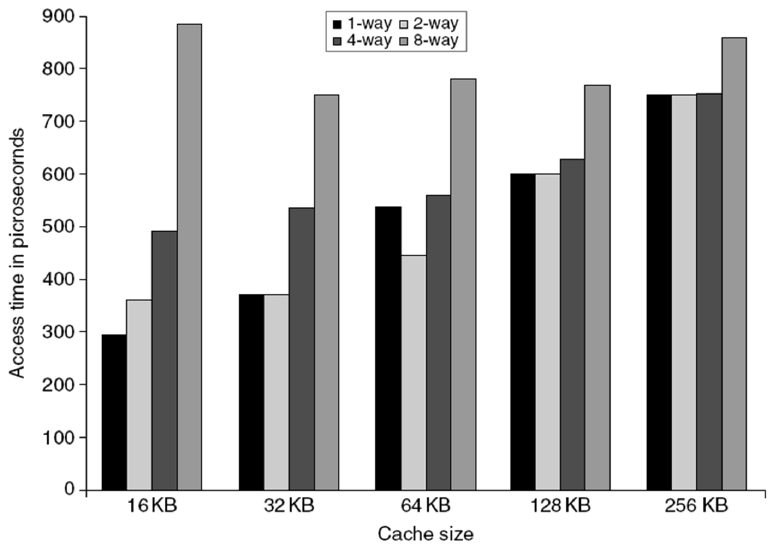
\includegraphics[scale=0.5]{img/hittimel1.png}
\caption{Tempi di hit per dimensione e livello di associatività di una cache.}\label{fig:hittimel1}
\end{figure}
Un'altra tecnica per ridurre il tempo di hit è quella di risolvere il problema della traduzione degli indirizzi. Ogni qualvolta la CPU effettua un cambio di contesto ovvero passa all'esecuzione di un altro processo è necessario svuotare la cache altrimenti si otterrebbero dei falsi hit. Una soluzione è quella di permettere che ogni blocco cache ha solo un indirizzo fisico che corrisponde agli n bits meno significativi di quelli virtuali, questa tecnica è chiamata \emph{page coloring}.
Per risolvere il problema del flush della cache è quello di aggiungere un tag identificativo del processo per verificare che il blocco al quale si sta accedendo appartenga al processo in esecuzione.\\
Un'idea per incrementare la velocità di hit è quella di inserire una pipeline per effettuare il check del tag e aggiornare i dati in cache in due stage diversi così facendo si aumenta il throughput del sistema tuttavia aumenta anche la penalità in caso di predizione errata di un salto.\\
L'ultima tecnica si pone l'obiettivo di ridurre il tempo di write e si basa sull'idea che la maggior parte degli update avviene su una porzione molto piccola del blocco di cache, solitamente una \emph{parola} per tale motivo è utile effettuare gli update solo di sotto-blocchi di dimensione di una parola.\\
Per un ricapitolazione delle diverse tecniche rimandiamo alla \figurename\,\ref{fig:performancerecap} nella quale si mostrano i vantaggi e gli svantaggi nonché la complessità delle diverse soluzioni
\begin{figure}[htb]
\centering
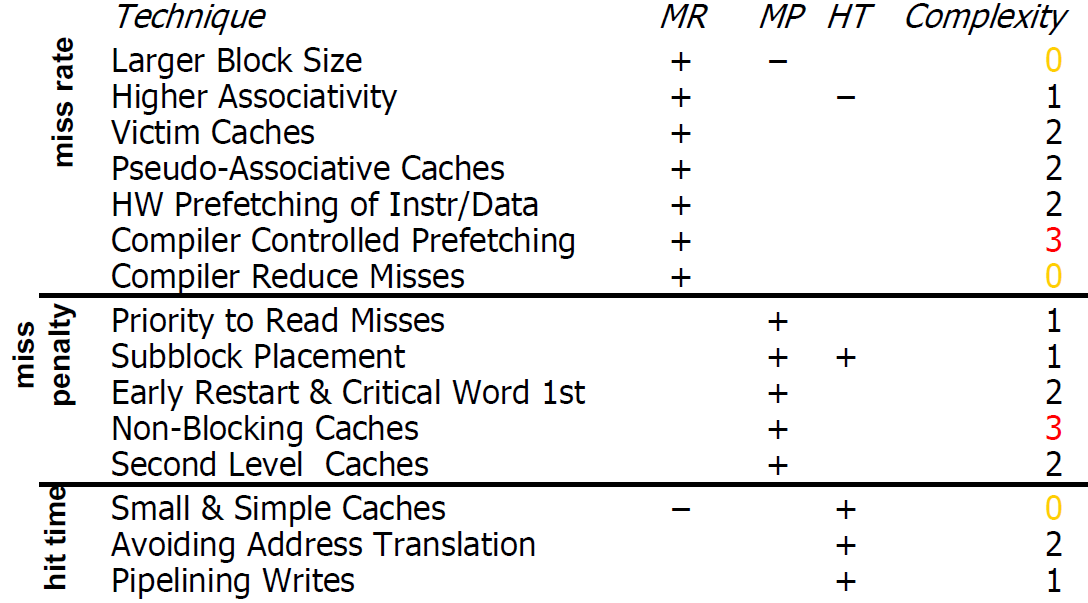
\includegraphics[scale=0.5]{img/performancerecap1.png}
\caption{Principali tecniche di incremento delle performance}\label{fig:performancerecap}
\end{figure}

\begin{figure}[htb]
\centering
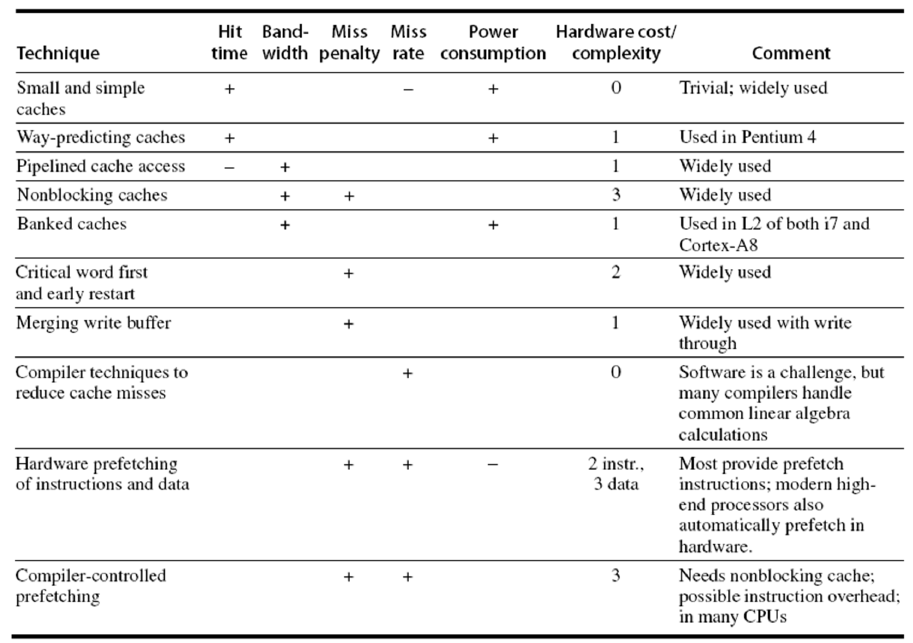
\includegraphics[scale=0.5]{img/performancerecap2.png}
\caption{Principali tecniche di incremento delle performance}
\end{figure}
\subsection{Virtual Memory}
La memoria virtuale è un meccanismo che serve a tradurre gli indirizzi virtuali in indirizzi fisici, ovvero ad effettuare il \emph{memory mapping}. Praticamente la memoria virtuale è un meccanismo che tratta la memoria come una cache per il disco in questo caso però i blocchi vengono chiamati \emph{pagine}.\\
Il concetto di memoria virtuale è stato introdotto innanzitutto per separare lo spazio degli indirizzi del processore dalla dimensione reale della memoria fisica come mostrato in \figurename\,\ref{fig:virtualtrans}
\begin{figure}
\centering
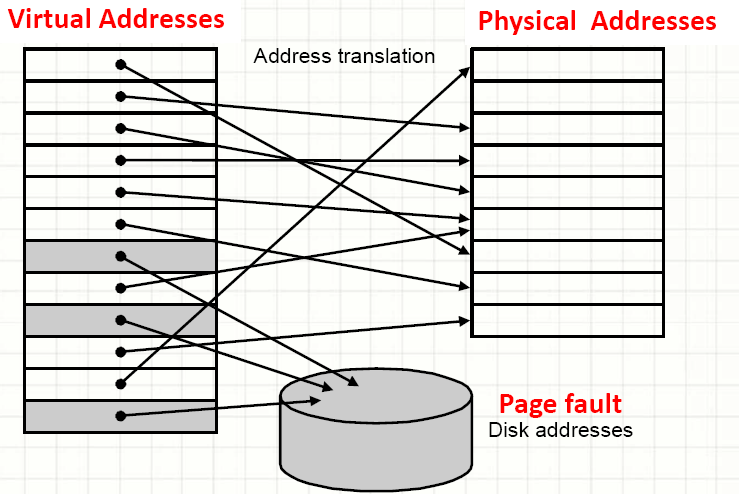
\includegraphics[scale=0.4]{img/virtualtrans.png}
\caption{Traduzione da indirizzo virtuale ad uno fisico}\label{fig:virtualtrans}
\end{figure}
Il meccanismo di traduzione da indirizzo virtuale ad indirizzo reale è basato su una \emph{Page Table} che viene associata ad ogni processo, ogni processo ha una sua page table e le page table di tutti i processi risiedono nella memoria fisica. Ogni page table mappa il \emph{virtual page number (VPNs)} con il rispettivo \emph{physical page number (PPNs)}, il VPN viene utilizzato come indice della \emph{page table}. Un esempio di page table è mostrato in \figurename\,\ref{fig:pagetable} in tale esempio vediamo anche come sia presente per ogni record della tabella un bit di validità per distinguere quale di queste pagine sono presenti in memoria (bit di validità a 1) oppure immagazzinate sul disco (bit di validità a 0).
\begin{figure}
\centering
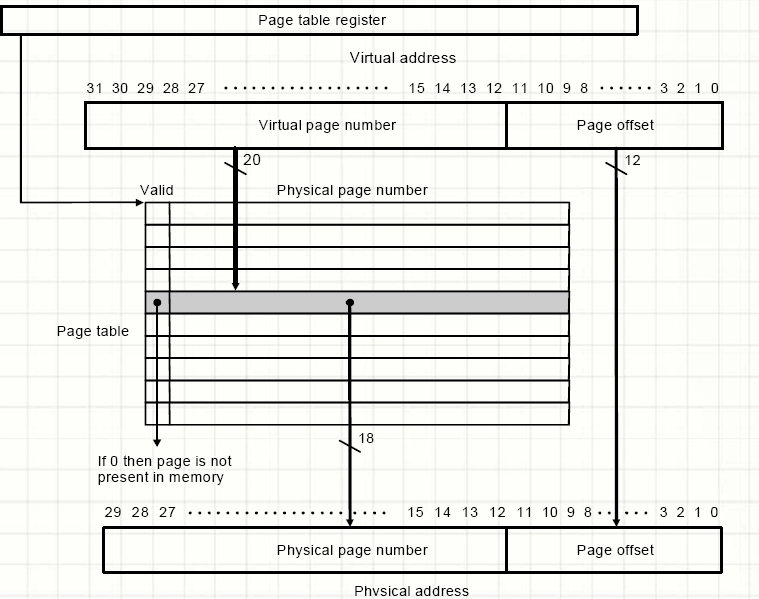
\includegraphics[scale=0.5]{img/pagetable.png}
\caption{Esempio di page table}\label{fig:pagetable}
\end{figure}
\subsubsection{Memory managment unit}
Per incrementare le performance l'idea è quella di inserire una cache per velocizzare la traduzione degli indirizzi. Questa particolare cache prende il nome \emph{Translation Look-Aside Buffer} ed è una piccola cache di circa 128-256 entità di tipo completamente associativo.
Cosa succede in caso di miss nella TLB, nel caso di soluzione hardware lo hardware della MMU la controlla la page table corrente e nel caso di entità valida la trasferisce alla TLB in caso contrario comunica al kernel il \emph{page fault}. Nel caso di soluzione software il processore riceve il TLB fault il kernel ritrova il record nella corrispettiva page table, nel caso di entità valida viene restituita l'entità in caso contrario il kernel richiama internamente la procedura di page fault.